\documentclass[12pt]{article}
\usepackage[english]{babel}
\usepackage[utf8x]{inputenc}
\usepackage{amsmath}
\usepackage{tablefootnote}
\usepackage{amssymb}
\usepackage{graphicx}
\usepackage{float}
\usepackage[colorinlistoftodos]{todonotes}
\usepackage{geometry}
\usepackage{booktabs}
\usepackage{siunitx}
\usepackage{subcaption}
\geometry{a4paper, margin=1in}
\usepackage{tabularx}
\usepackage{placeins}


\usepackage[style=authoryear, backend=biber, hyperref=true, citestyle=authoryear-comp]{biblatex}
\usepackage[colorlinks=true, linkcolor=blue, citecolor=blue, urlcolor=blue]{hyperref}
\hypersetup{
    colorlinks=true,
    linkcolor=blue,
    citecolor=blue,
    urlcolor=blue
}
\addbibresource{bibli.bib}
\geometry{letterpaper, margin = 2 cm}

% Set the depth for numbering sections
\setcounter{secnumdepth}{4}

\begin{document}



\newcommand{\HRule}{\rule{\linewidth}{0.5mm}} 

\thispagestyle{empty}

\begin{center}


\includegraphics[width=0.45\textwidth]{amse_logo.png}\\
\vspace{0.5cm}
\textsc{\huge Aix Marseille School of Economics} \\[0.3cm]

\vspace{2cm}


\textsc{\LARGE Final Evaluation in the courses of}\\[0.4cm]
\textsc{\large Predictive Methods}\\[0.1cm]
\textsc{\large Machine \& Statistical Learning,} \\[0.1cm]
\textsc{\large Information Reduction Methods}


\vspace{1cm}


\HRule \\[0.4cm]
{ \huge \textbf{Car Price Prediction} \\[0.5cm] 
Development of a mixed machine learning model to predict car prices
}\\[0.4cm]
\HRule \\[3cm]


\begin{minipage}[t]{0.8\textwidth}
	\begin{itemize}
    \item[\emph{Authors:}] Honorine DESILLES, \\
    Olivier JAYLET, \\
    Marcel PENDA 
    \item[\emph{Program:}] M.Sc. Econometrics, Big Data and statistics
	\item[\emph{Professors:}] Pierre MICHEL, \\ Sullivan HUE
	\item[\emph{Submission:}] \today
	\end{itemize}
\end{minipage}




\end{center}
\newpage

\renewcommand{\contentsname}{Table of contents}\tableofcontents

\newpage

\section{Introduction}



A detailed introduction specifying your objective and your approach to address it. The study must
be motivated by your knowledge as an economist. The introduction should allow the reader to
answer the following points:
- what you are focusing on
- why it is relevant (think as economists here)
- what is already known in the literature (and why it needs attention)
- how you address the question (here, using an empirical analysis)
- what you specifically did (strategy and methods, in a nutshell)
- what you found (highlight of your key results)
Ideally, you should be able to cite in your introduction academic articles that propose a topic related
to the one you are studying.




Problem: Due to lower prices, the reselling of cars has always been an interesting market for potential car buyers. However, the risk of buying a malfunctioning car exists...
Technology and new concepts such as internet providers, sharing economy applications for car sharing or online marketplaces such as leboncoin or ebay have facilitated the process of matching sellers and buyers. Companies such as Autobiz Car24 etc. are specializing in providing online platforms for reselling cars. However, price estimation is very difficult when evaluating used cars based on basic characteristics such as model, horse power, kilometers run etc..
Solution: Developing a solution based on different machine learning models that use basic car  characteristics and image data to estimate an adequate market price of a car of interest.



\section{Materials and Methods}
\subsection{Database}

Notre projet se compose de deux bases de données distinctes : une première contenant des données numériques et catégoriques et une seconde constituée d'images. Dans cette section, nous commencerons par présenter la première base de données, puis nous décrirons la seconde base de données.

\subsubsection{Categorical and numerical data}

\paragraph{Data Description}
~~\\
\\
Afin de créer un dataset comprenant des données numériques et catégoriques, nous avons décidé de fusionner deux bases de données misent à notre  disposition, comme indiqué dans le "voir papier". \\

\noindent La première table se nomme Ad table. C'est un dataset qui comprend 268,255 observations et 24 variables. Ces variables décrivent les caractéristiques des véhicules comme la taille, la couleur, le prix, le modèle, etc. Ces données peuvent être des données catégoriques telles que le fabricant de la voiture, le modèle ou le type de boite de vitesse. Il y a également des données numériques telles que la puissance du moteur, le prix. De nombreuses données manquantes sont présentes dans cette table notamment dans les colonnes couleurs, la taxe annuel, le mpg moyen ou le top speed. Nous expliquerons dans la section suivante, qui se nomme préprocessing comment nous avons gérer ces données manquantes. En outre, des outliers ont été identifiées dans cette table qui peuvent être dues à un problème de données mal renseignées ou la présence de modèles de voitures uniques et très différents des autres. Ces anomalies seront examinées de manière approfondie dans le preprocessing des données. \\

\noindent La seconde table se nomme Trim.csv. Cette table est composée de 335,562 observations et 9 variables. Nous avons seulement la variable permettant de savoir les émissions de gaz des voitures. \\

\noindent Suite à la jointure de ces deux tables nous avons obtenu une table finale de 213K observations avant le preprocessing. L'objectif de notre travail étant de prédire le prix des voitures notre dependant variable sera la variable "price". \\

\noindent Voici le dictionnaire des variables que nous avons sélectionné pour notre dataset final.

\begin{table}[ht]
    \centering
    \caption{Dictionary of Variables}
    \label{tab:variables}
    \begin{tabularx}{\textwidth}{lclX}
        \toprule
        \textbf{Variable} & \textbf{Type} & \textbf{Description} \\
        \midrule
        Price & Float & Prix du véhicule. \\
        Runned\_Miles & Float & Miles parcourus par le véhicule. \\
        Engin\_size & Float & Taille du moteur du véhicule. \\
        Engine\_power & Float & Puissance du moteur du véhicule. \\
        Wheelbase & Float & Empattement du véhicule. \\
        Height & Float & Hauteur du véhicule. \\
        Width & Float & Largeur du véhicule. \\
        Length & Float & Longueur du véhicule. \\
        Average\_mpg & Float & Consommation moyenne de carburant en miles par gallon. \\
        Gas\_emission & Float & Émission de gaz du véhicule. \\
        Top\_speed & Float & Vitesse maximale du véhicule. \\
        Seat\_num & Int & Nombre de sièges dans le véhicule. \\
        Door\_num & Int & Nombre de portes du véhicule. \\
        Body\_type & String & Type de véhicule. \\
        Gear\_box & String & Type de boîte de vitesse. \\
        Fuel\_type & String & Type de carburant. \\
        \bottomrule
    \end{tabularx}
\end{table}

\paragraph{Data Prepossessing}
~~\\

\noindent Afin de faire le preprecessing de manière uniforme et structurée nous avons opté pour l'utilisation de la programmation orientée objet (POO). C'est une méthode qui permet de créer des classes afin de créer et de manipuler des objets, ici les observations. Cette classe qui se nomme preprocess Ad Table Trim a permis un preprocessing efficace et optimisé (à voir). Dans un premier temps, nous avons renommé les colonnes de la table fusionnée afin d'avoir des noms de colonnes normalisés pour avoir la même structure pour toutes les variables. Ensuite, après une analyse des valeurs manquantes, nous avons decidé de les supprimer considérant notre base de données déjà très large et complète. Pour certaines variables, telles que "average mpg", "engine size", "engine power" et "top speed", nous avons décidé d'imputer les valeurs manquantes par la moyenne spécifique pour chaque type de modèle. Nous avons fait ce choix étant donné qu'il y avait beaucoup de valeurs manquantes dans ces variables qui nous semblaient très importantes dans notre base de données. \\

\noindent Ensuite, nous avons convertit toutes les données catégoriques en format numérique grâce à la fonction "one hot encoding" qui permet de créer des variables binaires, facilitant l'intégration de ces informations dans les modèles d'apprentissage automatique. Après avoir identifié les outliers (montrer quelques calculs ou graphs), nous avons supprimé les 1\% des prix les plus élevés et les données ayant des zscores supéireurs à 4. Le score est un calcul (mettre calcul) qui permet d'attribuer un score aux valeurs qui paraissent aberrantes. Cette étape a conduit à la suppression d'environ 10K observations, représentant x\% de notre base de données initiale. (voir pour le nombre de NaN supprimées).\\
Enfin, la dernière étape a été la standardization (calcul) des valeurs, c'est une étape primordiale en machine learning. Cela permet d'avoir des données sur une échelle commune, les rendant comparables. \\

\noindent Grâce à la création de cette classe automatisée, nous obtenons une classe qui assure la création d'un ensemble de données cohérent, prêt à être exploité pour l'entrainement des modèles de machine learning.\\



\noindent \textbf{Open Questions}
\begin{itemize}
    \item Should we use information reduction methods for ML models on classical data?
\end{itemize}
\paragraph{Descriptive Statistics}
~~\\

\noindent Les statistiques descriptives permettent d'obtenir une meilleure vue d'ensemble de notre base de données. 

\noindent Dans un premier temps, observons les variables numériques. La table de fréquence suivante permet de présenter les principales stats descriptives de ces variables avec le nombre de valeurs, la moyenne, l'écart-type, le minimum, le maximum et les quartiles. Cela nous permet d'avoir une idée de la distribution de ces variables.

\begin{table}[h]
    \centering
    \caption{ Descriptive statistics}
    \begin{tabular}{lrrrrrrr}
    \toprule
           & Price & Runned\_Miles & Engin\_size & Engine\_power & Height & Width & Length \\
    \midrule
     count & 200676 & 200676 & 200676 & 200676 & 200676 & 200676 & 200676 \\
     mean & 10589.9 & 52352.4 & 1.8085 & 137.959 & 1535.76 & 1885.63 & 4334.15 \\
     std & 9496.06 & 39580.4 & 0.600646 & 60.2528 & 116.157 & 149.073 & 402.895 \\
     min & 100 & 2 & 0.66 & 50 & 1112 & 1475 & 2727 \\
     25\% & 3995 & 18250 & 1.4 & 99 & 1460 & 1770 & 4052 \\
     50\% & 7950 & 46000 & 1.6 & 120 & 1495 & 1875 & 4344 \\
     75\% & 13799 & 80000 & 2 & 168 & 1615 & 2013 & 4644 \\
     max & 56750 & 222000 & 4.6 & 429 & 1951 & 2365 & 5970 \\
    \bottomrule
    \end{tabular}
\end{table}

\begin{table}[h]
    \centering
    \begin{tabular}{lrrrrrrr}
    \toprule
           & Average\_mpg & Top\_speed & Gas\_emission & Wheelbase & Seat\_num & Door\_num \\
    \midrule
     count & 200676 & 200676 & 200676 & 200676 & 200676 & 200676 \\
     mean & 51.9473 & 120.585 & 152.543 & 2636.89 & 4.92767 & 4.45066 \\
     std & 12.3794 & 15.6977 & 37.9909 & 169.992 & 0.790823 & 0.931608 \\
     min & 9.8 & 80 & 0 & 1445 & 1 & 2 \\
     25\% & 43.5 & 109 & 129.096 & 2511 & 5 & 4 \\
     50\% & 51.4 & 118 & 142.786 & 2634 & 5 & 5 \\
     75\% & 61.1608 & 130 & 167.316 & 2741 & 5 & 5 \\
     max & 134.5 & 189 & 440 & 4065 & 9 & 5 \\
    \bottomrule
    \end{tabular}
\end{table}

\FloatBarrier

\noindent Interpretation: En moyenne une voiture coute 10 589.90€. (en italique) \\

\\

\noindent Le graphique suivant (Figure 1) illustre la distribution de notre target variable, le prix. Ce boxplot révèle une distribution resserrée, indiquant que la plupart des données sont concentrées entre 5 000 et 10 000€, avec une faible dispersion. La médiane, représentée par la ligne centrale de la boîte, se situe à 9 000€, signifiant que 50\% des données sont inférieures à cette valeur.
\noindent Les moustaches du graphique, généralement associées aux valeurs extrêmes, présentent des points sur la partie droite après la moustache droite, identifiés comme outliers. Malgré des efforts pour nettoyer la variable prix, réduisant la plage des valeurs de 100 000€ à 56 000€, le graphique met en évidence la persistance de nombreux outliers. Par choix, nous avons décidé de conserver ces valeurs, considérées comme moins aberrantes que celles de notre dataset initial.
\noindent Ce box plot montre une asymétrie dans la distribution de notre variable dépendante.

\FloatBarrier
\begin{figure}[ht]
    \centering
    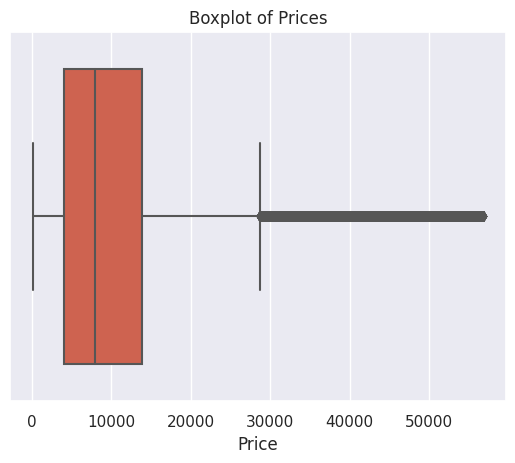
\includegraphics[width=0.45\textwidth]{boxplot price.png}
    \caption{Boxplot of prices}
    \label{fig:boxplot}
\end{figure}
\FloatBarrier

\noindent Ensuite, nous avons décidé de montrer la relation entre chaque variable numérique de type float avec le prix. Cette représentation graphique s'est avéré utile pour détecter des outliers dans un premier temps, que nous avons supprimé dans l'étape de préprocessing précédemment expliqué. Cela peut également être intéresant d'étudier la répartition des prix pour chaque variable afin de se familiariser avec le dataset que nous utiliserons ultérieurement pour entrainer nos modèles. Enfin, cette approche nous permet de d'identifier des tendances entre les variables indépendantes et la variable dépendante, le prix. Par exemple, nous pouvons observer une corrélation positive entre le prix des véhicules et la puissance du moteur.

\begin{figure}[ht]
    \centering
    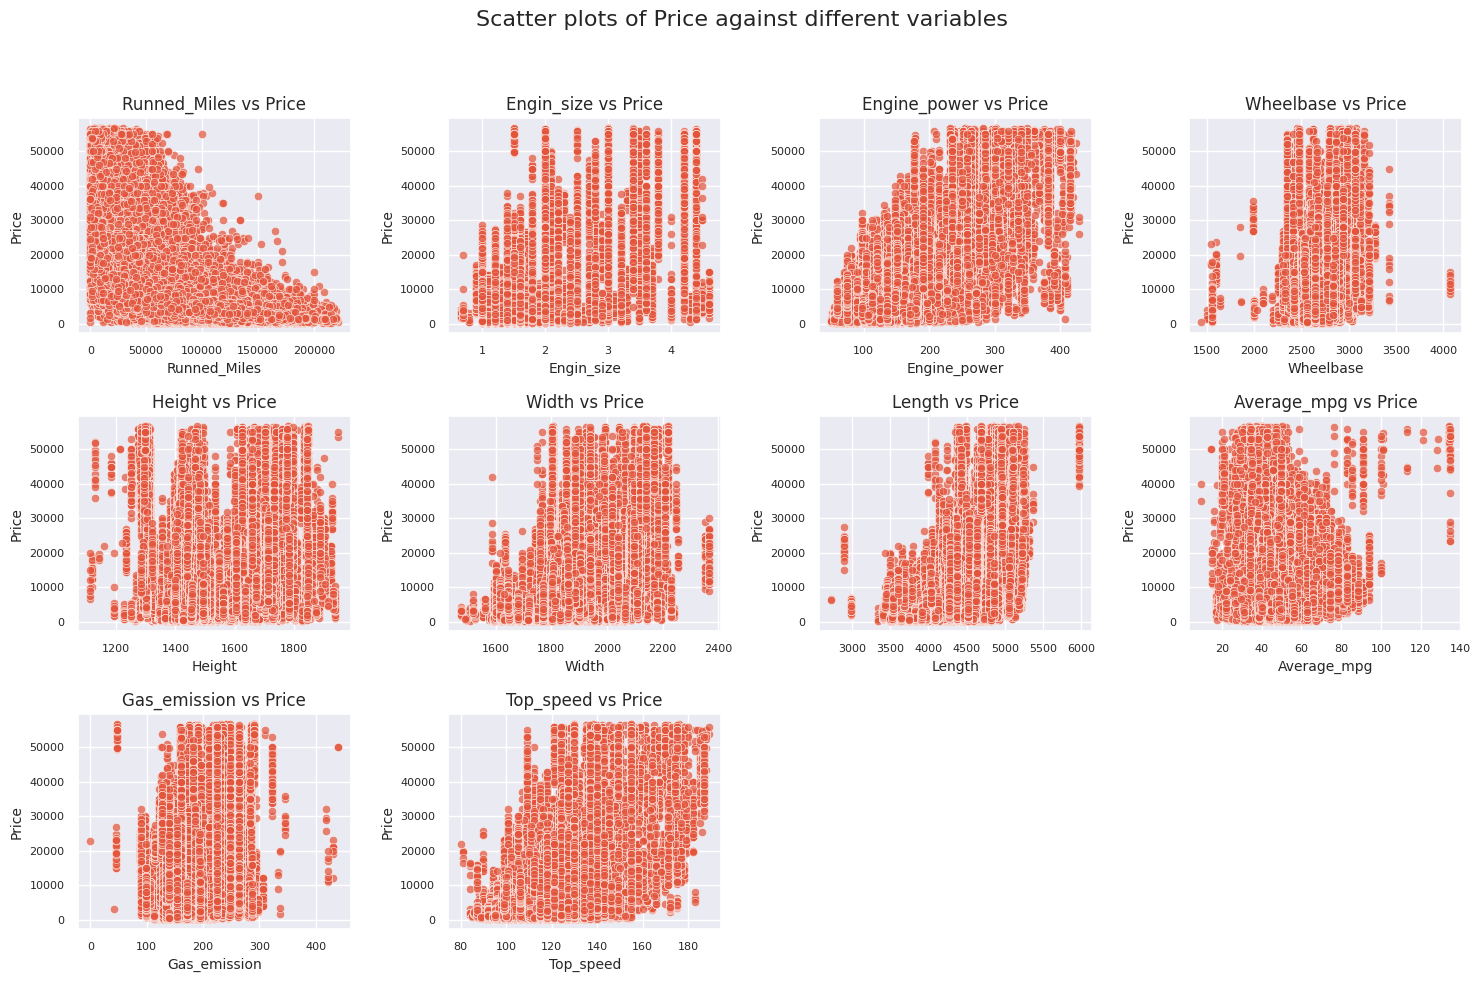
\includegraphics[width=0.95\textwidth]{numerique variables.png}
    \caption{Relationship between quantitative variables and the price}
    \label{fig:boxplot}
\end{figure}
\\
\FloatBarrier

Nous avons choisi d'utiliser des boxplots pour examiner la relation entre le prix des voitures et deux variables de type integer, afin que les graphiques soient plus compréhensibles. Après le preprocessing, nous avons constaté qu'il n'y avait plus que 4 valeurs possibles pour le nombre de portes. Parmi ces valeurs, les voitures à trois portes semblent moins dispersées. Concernant le nombre de sièges, une valeur aberrante persiste avec zéro siège, probablement due à une donnée mal renseignée. Par ailleurs, les données présentent des comportements très divergents en termes de prix en fonction du nombre de sièges. Par exemple, les modèles avec 2, 5, 7 et 8 sièges ont tendance à avoir un prix plus faible, ne dépassant jamais les 30 000 euros pour ces modèles.

\FloatBarrier
\begin{figure}[ht]
  \centering
  \begin{subfigure}{0.48\textwidth}
    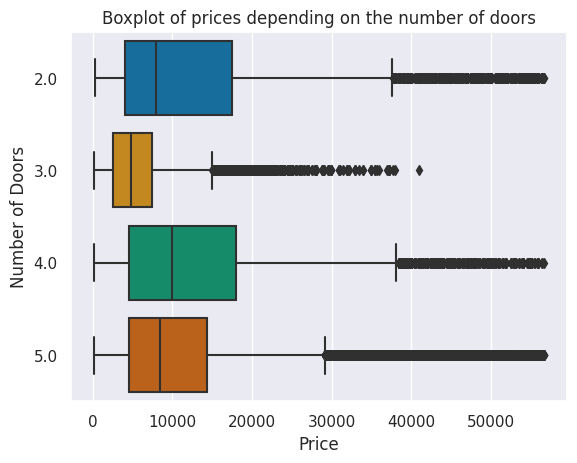
\includegraphics[width=\linewidth]{number of doors.png}
    \caption{Caption for Image 1}
    \label{fig:image1}
  \end{subfigure}
  \hfill
  \begin{subfigure}{0.48\textwidth}
    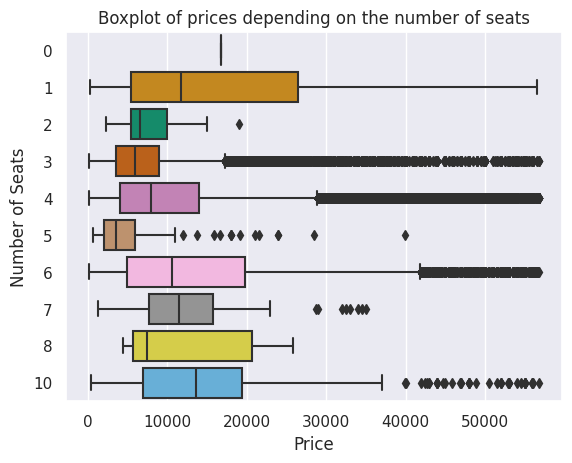
\includegraphics[width=\linewidth]{number of seats.png}
    \caption{Caption for Image 2}
    \label{fig:image2}
  \end{subfigure}
  \caption{Boxplots of prices depending on integer variables}
  \label{fig:twoimages}
\end{figure}
\FloatBarrier

\noindent Enfin, nous avons analysé les données qualitatives en utilisant également des boxplots. Le graphique de gauche a révélé des différences (significatives) dans la dispersion des données en fonction du type de carburant. Les boîtes à moustaches indiquent des variations marquées entre les différentes catégories de carburant, soulignant ainsi l'impact potentiel de cette variable sur la prédiction du prix des véhicules. 
Le graphique au centre, associé aux types de véhicules a montré une répartition similaire pour les sept premiers types, tandis que les deux derniers types "Car Derived Van" et "Limousine" se distinguent nettement des autres en tendant vers des prix plus bas, probablement en raison d'une quantité de données réduite. 
Enfin, le dernier boxplot à droite a mis en évidence une tendance selon laquelle les voitures équipées d'une boîte de vitesses automatique ont tendance à être plus cheres que celles avec une boîte manuelle.

\FloatBarrier
\begin{figure}[ht]
  \centering
  \begin{subfigure}{0.36\textwidth}
    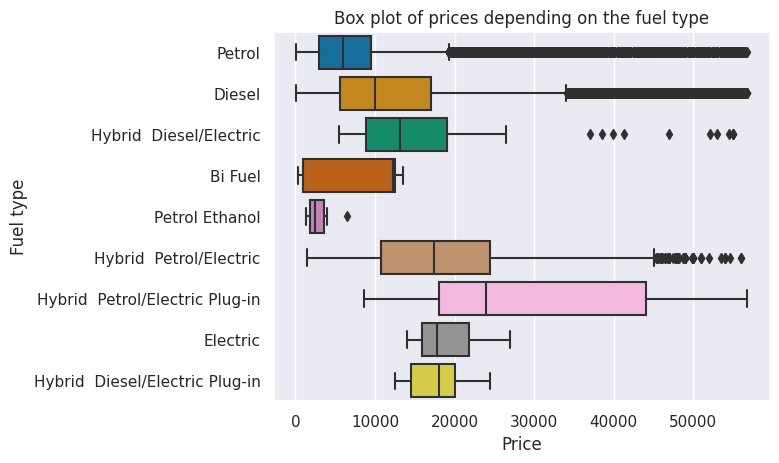
\includegraphics[width=\linewidth]{fuel type.png}
    \caption{Caption for Image 1}
    \label{fig:image1}
  \end{subfigure}
  \hfill
  \begin{subfigure}{0.32\textwidth}
    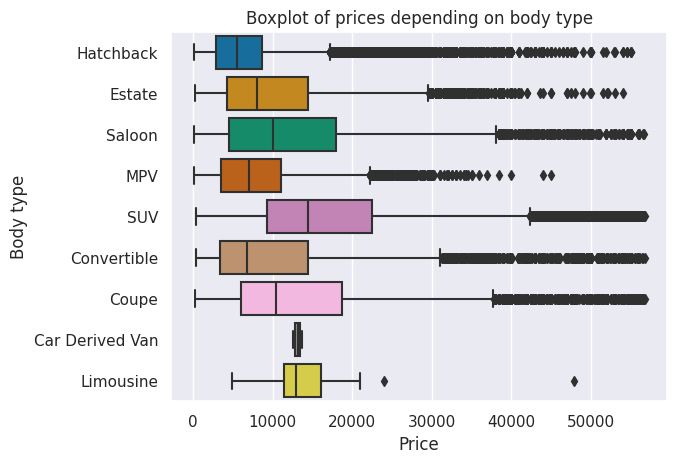
\includegraphics[width=\linewidth]{body type.png}
    \caption{Caption for Image 2}
    \label{fig:image2}
  \end{subfigure}
  \hfill
  \begin{subfigure}{0.30\textwidth}
    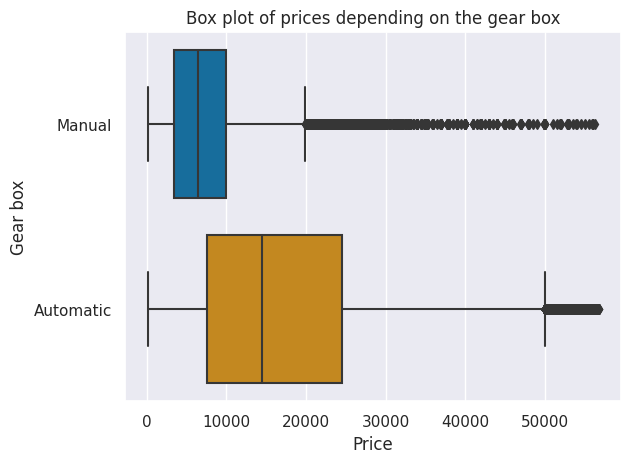
\includegraphics[width=\linewidth]{gear box.png}
    \caption{Caption for Image 3}
    \label{fig:image3}
  \end{subfigure}
  \caption{Dependance between qualitative variables and the price}
  \label{fig:threeimages}
\end{figure}
\FloatBarrier





\subsubsection{Image data}
\paragraph{Data Description}
~~\\
General information on data, source, tables etc. and explanation of potential outliers
\paragraph{Data Prepossessing}
~~\\
Removing outliers
\noindent \textbf{Open Questions}
\begin{itemize}
    \item Should we use information reduction methods for ML models on classical data?
\end{itemize}
\paragraph{Descriptive Statistics}
~~\\





mean, std, variance etc.
correlation matrix
We could include the PCA here, and then come back to it when we need it for our different models (e.e.g)
If we use PCA, we probably get a category dimensions (width, length, height), engine (size, horsepower etc.), condition (miles run, age etc.)

\subsection{Machine Learning Algorithms}
\subsubsection{Methods for Categorical and Numerical Data}
Short presentation / advantages and disadvantages / Reason of choice:
\begin{itemize}
    \item XGB
    \item SVM?
    \item Random Forest?
    \item GAM: Linear model and interpretable mixed with ridge or lasso (I think Sully said we should use at least one linear penalization  (irm) method. Also I think Flachaire presented a model: GAM ridge
    \item KNN?

L'algorithme K-nearest neighbors est un algorithme supervisé et non paramètrique. C'est-à-dire qu'il ne prend pas de fonction prédéfinie mais se construit à partir des données. Il peut être appliqué à des problèmes de classification ou de regression. Dans notre cas, pour déterminer les prix des voitures, nous utiliserons la classe KNeihborsRegresors du package scikit-learn. 
L'objectif de cet algorithme est de prédire la valeur d'une observation en faisant une moyenne des valeurs des k plus proches voisins. Générallement, la distance utilisée pour cet algorithme est la distance euclidienne (calcul) qui mesure la distance entre deux points dans l'espace des caractéristiques. L'enjeu majeur de cet algorithme étant de trouver le paramètre k optimal, celui qui minimise le taux d'erreur en prenant en compte le nombre de voisins qui permettent de prédire une valeur y, représentant la moyenne de ces voisins et étant le plus proche de la valeur initiale à prédire.

Dans un premier temps, nous avons cherché à optimiser k, représentant le nombre de voisins. Afin de déterminer cet hyperparamètre, nous avons entrainé le modèle KNN pour chaque k allant de 1 à 20. En comparant, le RMSE (root mean squared error) du train set et du validation set nous avons sélectionné la valeur de cet hyperparamètre. Le k qui minimise le RMSE du validation set avec un score de 1667 est 4. 

\FloatBarrier
\begin{figure}[ht]
    \centering
    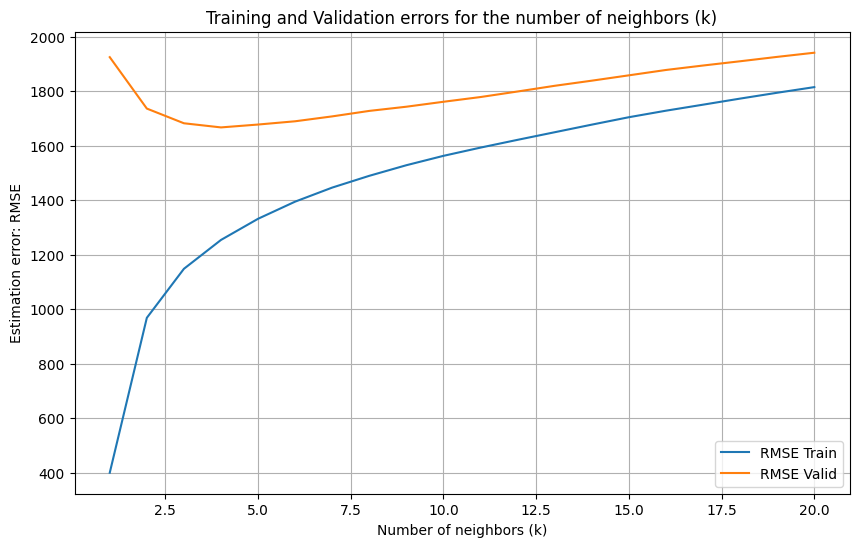
\includegraphics[width=0.45\textwidth]{Nb k.png}
    \caption{Training and Validation errors for the number of neighbors (k)}
    \label{fig:boxplot}
\end{figure}
\FloatBarrier

Après avoir sélectionné le modèle qui nous semblai le plus performant nous l'avons appliqué à notre test set pour voir le score sur des unseen data. Le score final est de 1719. 

\FloatBarrier
\begin{table}[h]
    \centering
    \begin{tabular}{lccc}
        \toprule
        \multirow{\textbf{Set}} & \textbf{RMSE} \\
        & \textbf{(k=4)} \\
        \midrule
        \textbf{Training} & 1254.05 \\
        \textbf{Validation} & 1667.01 \\
        \textbf{Test} & 1719.35 \\
        \bottomrule
    \end{tabular}
    \caption{KNN Model Results with k=4}
    \label{tab:knn_results}
\end{table}
\FloatBarrier

Afin de comprendre les variables qui étaient les plus déterminantes pour notre modèle nous avons appliqué la méthode des Shapley values, qui est modèle d'intélligibilité. C'est une technique qui a été dévéloppé en se basant sur la théorie des jeux en illustrant les joueurs comme des features, où chaque variable permet de contribuer à la valeur finale.

Après avoir appliqué la classe explainer du package Shap nous avons obtenu les données suivantes:


%\FloatBarrier
%\begin{figure}[ht]
%    \centering
%    \includegraphics[width=0.45\textwidth]{SHAP image.png}
%    \caption{Training and Validation errors for the number of neighbors (k)}
%    \label{fig:boxplot}
%\end{figure}
%\FloatBarrier

tatata... interpreter


Afin de réduire les dimensions de notre modèle nous avons utilisé la technique des partial component analysis. C'est une approche qui permet de réduire les dimensions d'un jeu de données tout en conservant la variance des données initiales. La base de données initiale, exprimée dans un espace de grande dimension sera réduit dans un espace de dimension inférieur, qui sera l'espace des composantes principales sélectionnées. 

Dans le but de choisir le nombre de dimensions que nous souhaitions nous avons créé le graphique suivant qui permet de visualiser la variance expliquée par chaque composante. Dans un objectif de 95\% de variance expliquée par notre nouveau jeu de données nous avons décidé de sélectionner les 10 premières composantes. Nous sommes ainsi passés de 33 variables à 13 composantes principales. 

\FloatBarrier
\begin{figure}[ht]
    \centering
    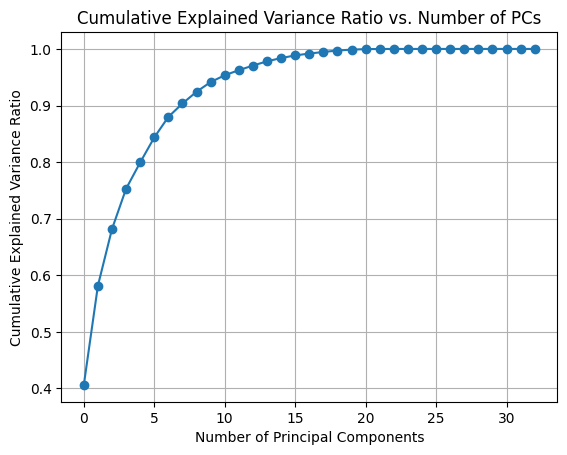
\includegraphics[width=0.45\textwidth]{PCA.png}
    \caption{Training and Validation errors for the number of neighbors (k)}
    \label{fig:boxplot}
\end{figure}
\FloatBarrier

Enfin, nous avons entraîné le modèle KNN sur l'ensemble d'entraînement transformé par la PCA et évalué ses performances sur l'ensemble de test.
Cela nous a permis de gagner du temps de traitement sans dégrader les résultats obtenus qui sont similiaires aux résultats du test avec l'ensemble des variables. (à continuer)








    \item PCA 
    \item PDP, SHAPLEY?
\end{itemize}


\subsubsection{Methods for image data}
Short presentation / advantages and disadvantages / Reason of choice:
\begin{itemize}
    \item CNN
    \item MLP
     \item PCA 
    \item PDP, SHAPLEY?
\end{itemize}

\subsubsection{Methods for mixed data}
\begin{itemize}
    \item Enter in hidden layers
    \item combine the data / models - but how?
\end{itemize}

\section{Results: Price estimation with classical data}
A detailed section: “Materials and Methods” presenting first the data used, the ways to collect and
format them; and a detailed description of the methods used in your analysis: theory elements on
the models used, empirical strategy (model selection, cross validation, grid search, etc.). Do not
forget to cite your sources.
Note: Your work should not be a catalogue of estimation methods. It is best to limit yourself to a
small number of methods, which you can present properly.

\subsection{Extreme Gradient Boosting Regression (XGBoost)}
\subsection{Support Vector Machines (SVM)}
\subsection{Model 3}
\subsection{Model 4}

\section{Results: Price estimation with image data}
\subsection{Convolution Neural Networks (CNN)}
\subsection{Multilayer Perceptron (MLP)}

\section{Results: Price estimation with mixed data}
\subsection{Selfmade model 1}
\subsection{Selfmade model 2}

\paragraph{CNN} 


Then we moved on the model that we wanted to apply to images data. The deep learning that take images data as input are called Convolutional Neural Network (litterature ?) CNN. The layers correspond to filter that we apply to a certain window of the image. They are composed of different steps, such as the convolution which the part that apply filter to the images, the pooling that reduces the dimension of the images by taking the mean of the a window for exemple or the dense layer also called the fully connected layer wich is ???. We wanted to build our own model but it was more complicated than we thought and it would take more time and lead to worst acuracy than a model that is already built. We knew about Alex-Net and Resnet but we wanted to take the last one in the "litterature". We decided to take Resnet16, which is an amelioration of Alexnet. The Alexnet was the first one developped for images challendes in 2012 (citer littérature). Restnet was introduced 3 years after in 2015 by Kaiming He, Xiangyu Zhang, Shaoqing Ren and Jian Sun in their paper “Deep Residual Learning for Image Recognition”. The particularity of this model is the residuality of the network, where his name come from. The difference with the previous model is that the result doesn't come from only from the output but from the difference between the input and the output like we can see in the following graph, what we called residual.



\FloatBarrier
\begin{figure}[ht]
    \centering
    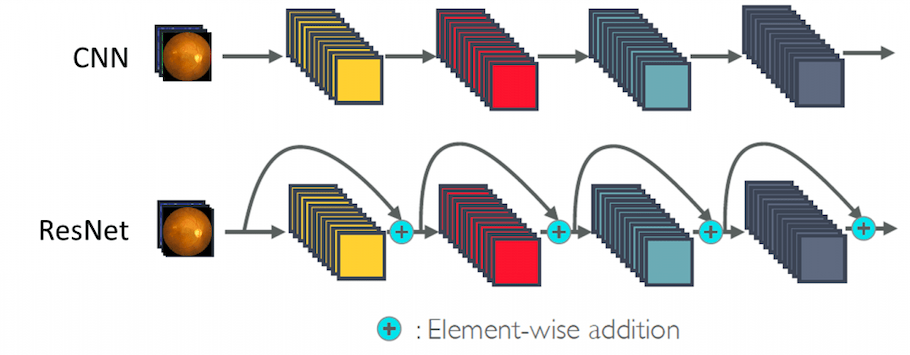
\includegraphics[width=0.45\textwidth]{CNN_RESNET}
    \caption{à faire}
    \label{fig:boxplot}
\end{figure}
\FloatBarrier

We selected the particular model Resnet16, because it's only composed of 16 layers which corresponds to the capacity of our machines. 

1 : input are rgb images of size 224 x 224
2 : first convolution 64 filters
3 : batch normalization sorte de rescaling pour faciliter le traitement du ML
4 :relu activation (déjà expliqué I guess)
5 : pooling which can be seen as a reduction methods bc it reduces the size of the images (résolution de l'image)
6 : enchainement de 4 residual blocs, each contains 2 convolution layers of ≠ size of filters, so in total 4*2=8 of basic blocks.
7 : global average pooling to reduce to a 1D
8 : fully connected for regression is not a softmax but a linear regression to have as output the predictions of our regression pb
nonnnn
t'es sur brouillon nonos
il a tjrs fonctionné lui
t'es teubé
my god
c'est pas ça le pb
mdrrrr
c'est fait depuis 23h hier ça

OUPS
PARDON
As rest18 is built to do a classification problem, we first need to delete the softmax activation function that does probabilities for the classes. In our case we will add a regression layer to obtain a prediction of the regression as an output. 

Question: 
Pourquoi as-tu choisi Resnet 18 ? : capacité de mémoire sur google colab pro
Expliquer en détails Resnet : toutes les couches
voir si les ≠ étapes n'ont pas été expliquées au dessus pour le MLP pour ne pas se répéter
expliquer les étapes qu'on a effectué (hyperpamètres ?)
learning rate et batch size ?

pretrained means and stds ? pourquoi et comment ? littérature qui cite ces variables ?

transformation des inputs ?

oulala le loader

les résultats obtenus

interprétabilité ?

besoin de faire de la réduction d'info en plus de l'étape de pooling ?





\section{Conclusion}
A conclusion recalling your major results and proposing possible future work and perspectives.






\end{document}
